\documentclass[10pt]{article}
\usepackage[paperwidth=8.5in, paperheight=11in, left=18mm, right=18mm, top=14mm, bottom=14mm]{geometry}
\usepackage{fontspec}
\usepackage{amsmath, amssymb}
\usepackage{xcolor}
\usepackage{graphicx}
\usepackage{tikz}
\usepackage{calc}

% Cài đặt font chữ chuẩn XeLaTeX
\IfFontExistsTF{TeX Gyre Termes}{\setmainfont{TeX Gyre Termes}}{}
\IfFontExistsTF{TeX Gyre Heros}{\setsansfont{TeX Gyre Heros}}{}

% Định nghĩa màu sắc theo chuẩn giáo trình Stewart Calculus
\definecolor{stewartblue}{RGB}{0, 136, 170}
\definecolor{stewartred}{RGB}{204, 37, 44}
\definecolor{examplecolor}{RGB}{0, 120, 140}
\definecolor{darkgraytext}{RGB}{80, 80, 80}

\pagestyle{empty}
\setlength{\parindent}{0pt}
\setlength{\parskip}{0pt}

\begin{document}

% Tiêu đề đầu trang (Running Header)
{\noindent\bfseries 254}\hspace{2.5em}{\bfseries CHƯƠNG 3}\hspace{1.2em}Các quy tắc đạo hàm
\par\vspace{10pt}

% Phần bài tập tiếp nối từ mục 3.9 (chia 2 cột đều nhau)
\noindent
\begin{minipage}[t]{0.485\textwidth}
  \fontsize{8.8pt}{11.5pt}\selectfont
  góc nâng là $\pi/3$, góc này đang giảm với tốc độ $\pi/6\text{ rad/phút}$. Khi đó máy bay đang bay với tốc độ bằng bao nhiêu?\par\vspace{8pt}
  
  \textbf{48.} Một vòng đu quay có bán kính $10\text{ m}$ đang quay với tốc độ một vòng mỗi $2\text{ phút}$. Một hành khách đang đi lên với tốc độ bao nhiêu khi chỗ ngồi của người đó ở độ cao $16\text{ m}$ phía trên mặt đất?\par\vspace{8pt}
  
  \textbf{49.} Một máy bay bay với tốc độ không đổi $300\text{ km/h}$ bay qua phía trên một trạm radar mặt đất ở độ cao $1\text{ km}$ và bay lên theo một góc $30^\circ$. Hỏi khoảng cách từ máy bay đến trạm radar tăng với tốc độ bao nhiêu sau đó một phút?\par\vspace{8pt}
  
  \textbf{50.} Hai người cùng xuất phát từ một điểm. Một người đi về hướng đông với vận tốc $3\text{ mi/h}$ và người kia đi về hướng đông bắc với vận tốc $2\text{ mi/h}$. Hỏi khoảng cách giữa hai người thay đổi với tốc độ bao nhiêu sau $15\text{ phút}$?
\end{minipage}\hfill
\begin{minipage}[t]{0.485\textwidth}
  \fontsize{8.8pt}{11.5pt}\selectfont
  \textbf{51.} Một vận động viên chạy nước rút quanh một đường chạy tròn bán kính $100\text{ m}$ với tốc độ không đổi $7\text{ m/s}$. Bạn của vận động viên đứng cách tâm đường chạy một khoảng $200\text{ m}$. Hỏi khoảng cách giữa hai người bạn thay đổi với tốc độ bao nhiêu khi khoảng cách giữa họ là $200\text{ m}$?\par\vspace{8pt}
  
  \textbf{52.} Kim phút trên một chiếc đồng hồ dài $8\text{ mm}$ và kim giờ dài $4\text{ mm}$. Hỏi khoảng cách giữa hai đầu kim thay đổi với tốc độ bao nhiêu vào lúc một giờ?\par\vspace{8pt}
  
  \textbf{53.} Giả sử thể tích $V$ của một quả cầu tuyết đang lăn tăng lên sao cho $dV/dt$ tỉ lệ thuận với diện tích bề mặt của quả cầu tuyết tại thời điểm $t$. Hãy chứng minh rằng bán kính $r$ tăng với tốc độ không đổi, nghĩa là $dr/dt$ là hằng số.
\end{minipage}

% Thanh tiêu đề Mục 3.10
\vspace{16pt}
\noindent
\begin{minipage}[b]{44mm}
  \raggedleft
  
\begin{tikzpicture}[baseline=0.5ex]
    \foreach \y in {0, 2.5, 5, 7.5, 10} {
      \draw[stewartblue, line width=0.8pt] (0, \y pt) -- (24pt, \y pt);
    }
  \end{tikzpicture}\hspace{6pt}%
  {\fontsize{21}{21}\selectfont\bfseries\sffamily\color{stewartblue} 3.10}%
  \hspace{6pt}%
  {\color{stewartblue}\rule[-3pt]{1.5pt}{21pt}}%
\end{minipage}%
\hspace{6mm}%
\begin{minipage}[b]{125mm}
  {\fontsize{16.5}{20}\selectfont\bfseries\sffamily Xấp xỉ tuyến tính và vi phân}
\end{minipage}

% Bố cục 2 cột bất đối xứng: Lề trái (Hình 1) và Nội dung chính
\vspace{10pt}
\noindent
\begin{minipage}[t]{44mm}
  \vspace*{68pt}
  \centering
  \IfFileExists{images/p0289_fig1.png}{%
    
\includegraphics[width=\linewidth]{images/p0289_fig1.png}%
  }{%
    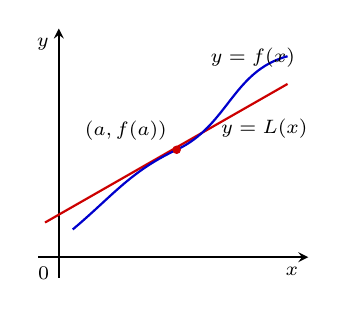
\begin{tikzpicture}[scale=0.88]
      \draw[->, >=stealth, line width=0.6pt] (-0.3,0) -- (3.6,0) node[below left, font=\scriptsize] {$x$};
      \draw[->, >=stealth, line width=0.6pt] (0,-0.3) -- (0,3.3) node[below left, font=\scriptsize] {$y$};
      \node[below left, font=\scriptsize] at (0,0) {$0$};
      \draw[red!80!black, thick] (-0.2, 0.5) -- (3.3, 2.5);
      \node[right, font=\scriptsize] at (2.2, 1.85) {$y=L(x)$};
      \draw[blue!80!black, thick] (0.2, 0.4) to[out=40, in=205] (1.7, 1.55) to[out=25, in=195] (3.3, 2.9);
      \node[above, font=\scriptsize] at (2.8, 2.6) {$y=f(x)$};
      \filldraw[red!80!black] (1.7, 1.55) circle (1.5pt);
      \node[above left, font=\scriptsize] at (1.7, 1.55) {$(a, f(a))$};
    \end{tikzpicture}%
  }
  \par\vspace{4pt}
  {\bfseries\sffamily\footnotesize HÌNH 1}
\end{minipage}%
\hspace{6mm}%
\begin{minipage}[t]{125mm}
  \fontsize{9.5pt}{12.5pt}\selectfont
  Chúng ta đã thấy rằng một đường cong nằm rất gần tiếp tuyến của nó ở lân cận tiếp điểm. Thật vậy, khi phóng to về phía một điểm trên đồ thị của một hàm khả vi, chúng ta nhận thấy đồ thị ngày càng giống với tiếp tuyến của nó. (Xem Hình 2.7.2.) Quan sát này là cơ sở cho phương pháp tìm các giá trị xấp xỉ của hàm số.\par\vspace{8pt}
  
  \noindent{\color{stewartblue}\rule{1.1ex}{1.1ex}}\hspace{0.5em}{\bfseries Tuyến tính hóa và xấp xỉ}\par\vspace{4pt}
  
  Việc tính giá trị $f(a)$ của một hàm số có thể dễ dàng, nhưng lại khó (hoặc thậm chí không thể) tính toán các giá trị lân cận của $f$. Vì vậy, chúng ta chọn các giá trị dễ tính hơn của hàm tuyến tính $L$ có đồ thị là tiếp tuyến của $f$ tại $(a, f(a))$. (Xem Hình 1.)\par\vspace{6pt}
  
  Nói cách khác, chúng ta sử dụng tiếp tuyến tại $(a, f(a))$ như một xấp xỉ cho đường cong $y = f(x)$ khi $x$ ở gần $a$. Phương trình của tiếp tuyến này là
  \[
  y = f(a) + f'(a)(x - a)
  \]
  Hàm tuyến tính có đồ thị là tiếp tuyến này, tức là,
  \par\vspace{4pt}
  \begin{center}
  
\begin{tikzpicture}
    \node[fill=stewartred, text=white, font=\bfseries\footnotesize, inner sep=2pt, minimum size=12pt] at (-4.6, 0) {1};
    \node[draw=stewartred, line width=0.8pt, inner xsep=20pt, inner ysep=5pt] at (0, 0) {$L(x) = f(a) + f'(a)(x - a)$};
  \end{tikzpicture}
  \end{center}
  \vspace{2pt}
  được gọi là \textbf{tuyến tính hóa} của $f$ tại $a$. Phép xấp xỉ $f(x) \approx L(x)$ hay
  \par\vspace{4pt}
  \begin{center}
  
\begin{tikzpicture}
    \node[fill=stewartred, text=white, font=\bfseries\footnotesize, inner sep=2pt, minimum size=12pt] at (-4.6, 0) {2};
    \node[draw=stewartred, line width=0.8pt, inner xsep=20pt, inner ysep=5pt] at (0, 0) {$f(x) \approx f(a) + f'(a)(x - a)$};
  \end{tikzpicture}
  \end{center}
  \vspace{2pt}
  được gọi là \textbf{xấp xỉ tuyến tính} hoặc \textbf{xấp xỉ bằng tiếp tuyến} của $f$ tại $a$.\par\vspace{8pt}
  
  \noindent{\bfseries\sffamily\color{examplecolor} VÍ DỤ 1}\hspace{0.8em}Tìm tuyến tính hóa của hàm số $f(x) = \sqrt{x + 3}$ tại $a = 1$ và dùng nó để xấp xỉ các số $\sqrt{3{,}98}$ và $\sqrt{4{,}05}$. Các xấp xỉ này là ước lượng thừa hay ước lượng thiếu?\par\vspace{6pt}
  
  \noindent{\bfseries\sffamily\color{examplecolor} LỜI GIẢI}\hspace{0.8em}Đạo hàm của $f(x) = (x + 3)^{1/2}$ là
  \[
  f'(x) = \frac{1}{2}(x + 3)^{-1/2} = \frac{1}{2\sqrt{x + 3}}
  \]
  và do đó ta có $f(1) = 2$ và $f'(1) = \frac{1}{4}$. Thay các giá trị này vào Phương trình 1, ta được
\end{minipage}

% Dòng chú thích bản quyền cuối trang
\vfill
\noindent
\begin{minipage}{\textwidth}
  \tiny\color{darkgraytext}
  Copyright 2021 Cengage Learning. All Rights Reserved. May not be copied, scanned, or duplicated, in whole or in part. WCN 02-200-203\\
  Editorial review has deemed that any suppressed content does not materially affect the overall learning experience. Cengage Learning reserves the right to remove additional content at any time if subsequent rights restrictions require it.
\end{minipage}

\end{document}